%Wave Maker Module

\subsubsection{Overview}
\label{Wave Maker}
\index{Wave Maker}\index{utilities, Wave Maker}

\begin{figure}[h]
\begin{center}
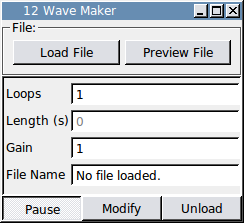
\includegraphics[width=2in]{wavemaker.png} 
\caption[Wave Maker]{The wave maker module allows the output of a pre-recorded signal from an ASCII file.} 
\end{center}
\label{wavemaker}
\end{figure}

The wavemaker module loads data from an ASCII formatted file. It samples one value from the file on every time step and generates an output signal. The module computes the time length of the waeform based on the current real-time period, set through the (\seealso{Chapter \ref{system control panel} \\System Control Panel}System Control Panel. User-generated modules can be tested using the wavemaker module, by simulating real-time acquisition of data.

\subsubsection{Output Channels}
\begin{description}
\item [Output]Values read from the ASCII file
\end{description}

\subsubsection{Parameters}
\begin{description}
\item [Loops]Number of times to repeat the waveform, looping back to the beginning
\item [Gain]Multiplicative gain to apply to the waveform values
\end{description}